\graphicspath{{3cyclic/asy/}}

\section{Cyclic groups}\label{chap:cyclic}

\subsection{Definitions and Basic Examples}\label{sec:cycdef}

Cyclic groups are a basic family whose complete structure is simple enough to be easily described. The foundational idea is that a cyclic group is generated by a single element.

\begin{examples}{}{cyclicexmotiv}
	\exstart $(\Z,+)$ is generated by 1: all integers may be produced by (repeatedly) combining 1 with itself using only the group operation ($+$) and inverses ($-$). For instance,
	  \[
	  	-4=-(1+1+1+1)
	  \]
	  %The identity may be constructed as $0=1+(-1)$.
	\begin{enumerate}\setcounter{enumi}{1}
	   \item The set of complex numbers $U_4=\{i,-1,-i,1\}=\{i,i^2,i^3,i^4\}$ is generated by the single element $i$ under multiplication. We'll revisit this example in more generality shortly.
	 	\item The group $R_n=\{\rho_0,\ldots,\rho_{n-1}\}$ of rotations of a regular $n$-gon (Definition \ref{defn:rotdiklein}) is generated by the `1-step' rotation $\rho_1$, since any other is just this repeated $\rho_k=\rho_1^k$.
	\end{enumerate}
\end{examples}

We formalize this idea by considering the subset of a group $G$ that may be produced starting with a single element $g$. Since we work abstractly, we follow the convention of writing $G$ multiplicatively.

\begin{lemm}{Cyclic subgroup}{cyclicdef}
	Let $G$ be a group and $g\in G$. The set
	\[
		\ip{g}:=\{g^n:n\in\Z\}=\{\ldots,g^{-1},e,g,g^2,\ldots\}
	\]
	is a subgroup of $G$. We call this the \emph{cyclic subgroup generated by $g$.}
\end{lemm}

\begin{proof}
	We follow the subgroup criterion (Theorem \ref{thm:subgroup}).
	\begin{quote}
		\emph{Non-emptiness}:\quad Plainly $e\in\ip g$.\par
		\emph{Closure}:\quad Every element of $\ip g$ has the form $g^k$ for some $k\in \Z$. The required condition follows from standard exponential notation: $g^k\cdot g^l=g^{k+l}\in\ip g$.\par
		\emph{Inverses}:\quad This is immediate by Exercise \ref*{sec:groupaxioms}.\ref{exs:multinverse2}: $(g^k)^{-1}=g^{-k}\in\ip g$.\qedhere
	\end{quote}
\end{proof}

\begin{defn}{Cyclic group}{cyclic}
	A group $G$ is \emph{cyclic} if it has a \emph{generator}: $\exists g\in G$ such that $G=\ip g$.\smallbreak
	In any group $G$, the \emph{order of an element $g$} is the order (cardinality) of the subgroup $\ip g\le G$.
\end{defn}

\textcolor{red}{Warning!} Don't confuse the \emph{order of a group} $G$ with the \emph{order of an element} $g\in G$. Cyclic groups are precisely those containing elements (generators) whose order equals that of the group!



\begin{examples*}{\ref{ex:cyclicexmotiv} cont}{}
	\exstart $\Z=\ip{1}=\ip{-1}$ is generated by either 1 or $-1$. As an additive group, the subgroup generated by 2 is the group of even numbers under addition
	\[
		\ip 2=\{\ldots,-2,0,2,4,\ldots\}=\{2m:m\in\Z\}=2\Z
	\]
	\begin{enumerate}\setcounter{enumi}{1}
	  \item $U_4=\ip{i}=\{1,i,-1,-i\}$ is a cyclic subgroup of $(\C^\times,\cdot)$. It is also generated by $-i$.
		\item $R_n=\ip{\rho_1}$. This group has other generators, but we'll delay describing them until the next section.
	\end{enumerate}
\end{examples*}
\goodbreak


\boldsubsubsection{Modular Arithmetic}

We introduce a family of finite groups based on the (hopefully familiar!) addition of remainders.

\begin{defn}{}{znsimple}
	Let $n$ be a positive integer. We denote by $\Z_n$ the set of \emph{equivalence classes of integers modulo $n$.} These are typically written as remainders
	\[
		\Z_n=\{0,1,\ldots,n-1\}
	\]
	where $x=y\in\Z_n$ means that the integers $x,y$ have the \emph{same remainder\footnotemark} on division by $n$.
\end{defn}

\footnotetext{%
	More formally, $x=y\in\Z_n$ means $x\equiv y\pmod n$, or equivalently $x=y+\lambda n$ for some integer $\lambda$. The elements of $\Z_n$ are strictly \emph{equivalence classes} where the equivalence class $[x]$ of $x\in\Z$ is the set of integers with the same remainder as $x$:
	\[
		[x]=\{z\in\Z:x\equiv z\negthickspace\pmod n\}=\{\ldots,x-n,x,x+n,x+2n\ldots\} =\{x+kn:k\in\Z\} =x+n\Z
	\]
	Addition of equivalence classes is \emph{well-defined}: if $[x]=[w]$ and $[y]=[z]$, then $w=x+\kappa n$ and $z=y+\lambda n$, from which
	\[
		[w]+_n[z]=[w+z] =\bigl[(x+\kappa n)+(y+\lambda n)\bigr] =\bigl[x+y+n(\kappa+\lambda)\bigr] =[x+y] =[x]+_n[y]
	\]
}

Several notations are available. For instance, here is a calculation in $\Z_5$ written four ways:\par
\begin{minipage}[t]{0.62\linewidth}\vspace{0pt}
	\begin{enumeratea}
	  \item Group/Number Theory style:\quad $4+2=6=1$ in $\Z_5$.
	  \item Modular arithmetic:\quad $4+2\equiv 6\equiv 1\pmod 5$.
	  \item Decorate the operation:\quad $4+_52=6=1$.
	  \item Equivalence classes:\quad $[4]+_5[2]=[6]=[1]$.
	\end{enumeratea}
	\textcolor{red}{Warning!}\quad For reasons of brevity we mostly use notation (a), though feel free to use another if you feel more comfortable. Regardless of notation, it \emph{must} be made clear in \emph{which} $\Z_n$ you are working: $4+2=1$ is not acceptable on its own!
\end{minipage}
\hfill
\begin{minipage}[t]{0.37\linewidth}\vspace{-12pt}
		\flushright%
		\begin{tabular}{@{}c@{}}
		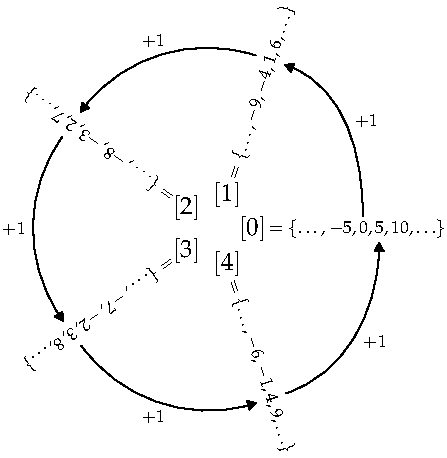
\includegraphics[scale=0.75]{cyclic-zn}\\
		Adding 1 in $\Z_5$\phantom{bo}
	\end{tabular}
\end{minipage}


\begin{thm}{}{zncyclic}
	$\Z_n$ forms a cyclic group of order $n$ under addition modulo $n$.
\end{thm}

A rigorous proof is tedious right now and will come for free in Chapter \ref{chap:coset} when $\Z_n$ is properly defined as a \emph{factor group.} For the present, note that $\Z_n$ is cyclic since it is generated by $1$: e.g.,
\[
	\Z_5=\ip 1=\{1,2,3,4,0\}=\{1,\ 1+1,\ 1+1+1,\ 1+1+1+1,\ 1+1+1+1+1\}
\]

\begin{examples}{}{}
	Here are the Cayley tables for $\Z_1,\Z_2,\Z_3,\Z_4$. Compare these to Example \ref*{ex:rx}.\ref{ex:smallcayley1}.
	\[
		\begin{array}[t]{c||c}
			+_1 & 0\\\hline\hline
			0 & 0
		\end{array}
		\qquad
		\begin{array}[t]{c||c|c}
			+_2 & 0 & 1\\\hline\hline
			0 & 0 & 1\\\hline
			1 & 1 & 0
		\end{array}
		\qquad
		\begin{array}[t]{c||c|c|c}
			+_3 & 0 & 1 & 2\\\hline\hline
			0 & 0 & 1 & 2\\\hline
			1 & 1 & 2 & 0\\\hline
			2 & 2 & 0 & 1
		\end{array}
		\qquad
		\begin{array}[t]{c||c|c|c|c}
			+_4 & 0 & 1 & 2 & 3\\\hline\hline
			0 & 0 & 1 & 2 & 3\\\hline
			1 & 1 & 2 & 3 & 0\\\hline
			2 & 2 & 3 & 0 & 1\\\hline
			3 & 3 & 0 & 1 & 2
		\end{array}
	\]
\end{examples}

The groups $\Z_n$ are typically those to which other cyclic groups are compared. Indeed in the next section we'll see that \emph{any} cyclic group of order $n$ is isomorphic to $\Z_n$!

\begin{example}{}{}
	$(\Z_3,+_3)$ is isomorphic to the rotation group $(R_3,\circ)$ via $\phi(k)=\rho_{k\pmod 3}$.
	\smallbreak
	It is worth doing this slowly, since the domain is a set of equivalence classes:
	\begin{quote}
		\emph{Well-definition}:\lstsp If $y=x\in\Z_3$, then $y\equiv x\equiv r\pmod 3$ for some $r\in\{0,1,2\}$. But then
		\[
			\phi(y)=\rho_r=\phi(x)
		\]
		\emph{Bijection}:\lstsp This is trivial $\phi:\{0,1,2\}\to\{\rho_0,\rho_1,\rho_2\}$.\par
		\emph{Homomorphism}:\lstsp This is the formula for composition of rotations
		$\rho_k\rho_l=\rho_{k+l\negthickspace\pmod 3}$
	\end{quote}
\end{example}



\boldsubsubsection{The Roots of Unity}

For a final family of cyclic groups, we consider subgroups of $(\C^\times,\cdot)$.

\begin{defn}{}{}
	Let $n\in\N$. The \emph{$n\th$ roots of unity} form the subgroup of $\C^\times$ generated by $\zeta:=e^{\frac{2\pi i}n}$:
	\[
		U_n:=\ip{\zeta}=\bigl\{1,\zeta,\zeta^2,\cdots,\zeta^{n-1}\bigr\}
	\]
\end{defn}

These are precisely the $n$ complex solutions to the equation $z^n=1$. To emphasize $n$, write $\zeta_n=\smash[t]{e^{\frac{2\pi i}n}}$. 


\begin{aside}
	\boldinline{Aside: Notation Review}
	
	In case you've not thought much about complex number notation, here is a \emph{brief} review. $\C=\{x+iy:x,y\in\R\}$ is the vector space $\R^2$ spanned by the basis $\{1,i\}$, where $i$ is a `number' satisfying $i^2=-1$. 
	Given $z=x+iy\in\C$, consider several objects:\par
	\begin{minipage}[t]{0.7\textwidth}\vspace{-4pt}
		\begin{description}\itemsep0pt
			\item[\normalfont\emph{Complex conjugate}:] $\cl z=x-iy$ is the reflection of $z$ in the real axis.
			\item[\normalfont\emph{Modulus (length)}:] $r=\nm z=\sqrt{z\cl z}=\sqrt{x^2+y^2}$.
			\item[\normalfont\emph{Argument (angle)}:] If $z\neq 0$, then $\theta=\arg z$ is the angle measured counter-clockwise from the positive real axis to the ray $\ray{0z}$.
			\item[\normalfont\emph{Polar form}:] $z=re^{i\theta} =r\cos\theta+ir\sin\theta$.
	\end{description}\vspace{-7pt}
	The modulus and argument are simply the usual polar co-ordinates of a point in $\R^2$. When $r=1$ we have \emph{Euler's formula}:
	\[
		e^{i\theta}=\cos\theta+i\sin\theta
	\]
	the source of the famous identity $\displaystyle e^{i\pi}=-1$. In the picture, $S^1$ denotes the \textcolor{Green}{unit circle}. Note also that\vspace{-2pt}
	\[
		e^{i\theta}=1\iff \theta=2\pi k\quad\text{for some integer $k$}\tag{$\dag$}
	\]
	The polar form behaves nicely with respect to multiplication:\vspace{-2pt}
	\end{minipage}
	\hfill
	\begin{minipage}[t]{0.29\textwidth}\vspace{-5pt}
		\flushright%
		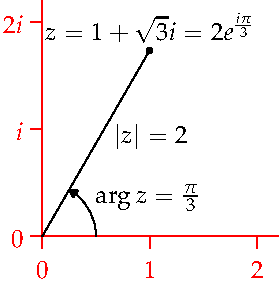
\includegraphics[scale=0.9]{cyclic-polar}\\
		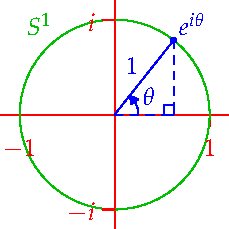
\includegraphics[scale=0.9]{cyclic-circle}
	\end{minipage}
	\par
	\[
		\nm{zw}=\nm z\nm w\quad \text{and}\quad \arg(zw)\equiv \arg z+\arg w \pmod{2\pi}
	\]
\end{aside}


\goodbreak


\begin{minipage}[t]{0.67\linewidth}\vspace{0pt}
	The square roots of unity are simply $\pm 1$, and we saw the $4\th$ roots $\pm 1,\pm i$ in Example \ref{ex:cyclicexmotiv}. More generally, the $n\th$ roots are form the vertices of a regular $n$-gon centered at the origin; this is since
	\[
		\nm{\zeta^k}=\nm\zeta^k=1
		\quad\text{and}\quad
		\arg\zeta^k=\arg e^{\frac{2\pi k}{n}}=\tfrac{2\pi k}n=k\arg\zeta
	\]
	We stop listing the elements of $U_n$ at $\zeta^{n-1}$, since $\zeta^n=e^{2\pi i}=1$. By $(\dag)$, we see a simple relationship with modular arithmetic:
	\[
		\zeta^k=\zeta^l\iff 1=\zeta^{k-l}=e^{\frac{2\pi i(k-l)}n}\iff k\equiv l\pmod n
	\]
\end{minipage}
\hfill
\begin{minipage}[t]{0.24\linewidth}\vspace{0pt}
	\centering
	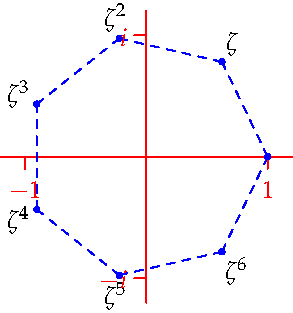
\includegraphics[scale=0.8]{cyclic-rootunity}\\
	Seventh roots: $\zeta_7=e^{\frac{2\pi i}7}$
\end{minipage}
\bigbreak

% 
% \begin{lemm}{}{}
% 	The $n\th$ roots of unity are precisely the $n$ (complex) roots of the equation $z^n=1$.\
% \end{lemm}
% 
% \begin{proof}
% 	Plainly $(\zeta^k)^n=(e^{\frac{2\pi ik}n})^n=e^{2\pi ik}=1$, so every element of $U_n$ solves $z^n=1$.\smallbreak
% 	For the converse, suppose $z^n=1$. Take the modulus to obtain $\nm{z}^n=1$. Since $\nm{z}$ is a non-negative real number, we see that $\nm{z}=1$, whence its polar form is $z=e^{i\theta}$. Now compute:
% 	\[
% 		1=z^n=(e^{i\theta})^n=e^{in\theta}\iff n\theta=2\pi k
% 	\]
% 	for some integer $k$ ($\ast$). But then $\theta=\frac{2\pi k}n$ and so
% 	\[
% 		z=e^{i\theta}=e^{\frac{2\pi i}nk}=\left(e^{\frac{2\pi i}n}\right)^k=\zeta^k\tag*{\qedhere}
% 	\]
% \end{proof}

\begin{examples}{}{unisoex}
	\exstart Observe that $\zeta_6^2=(e^{\frac{2\pi i}6})^2 =e^{\frac{2\pi i}3} =\zeta_3$.\par
	\begin{enumerate}\setcounter{enumi}{1}
		\begin{minipage}[t]{0.75\linewidth}\vspace{-4pt}
			\item[]This immediately results in a subgroup relationship: with $\textcolor{blue}{\zeta}=\zeta_6$, 
			\[
				U_3 = \bigl\{\textcolor{red}{1},\textcolor{red}{\zeta^2},\textcolor{red}{\zeta^4}\bigr\}  < U_6 = \bigl\{\textcolor{red}{1},\zeta,\textcolor{red}{\zeta^2},\zeta^3,\textcolor{red}{\zeta^4},\zeta^5\bigr\}
			\]
			This is essentially trivial from a picture (compare Example \ref{ex:hexsubgroup}).
		\end{minipage}
		\hfill
		\begin{minipage}[t]{0.24\linewidth}\vspace{-30pt}
			\flushright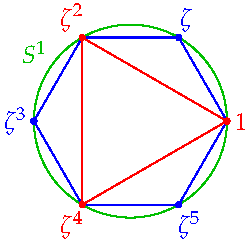
\includegraphics[scale=0.8]{cyclic-hexagon}
		\end{minipage}
	  
	  
	  \item\label{ex:unisoex2} Cayley tables for $U_n$ are simple to construct. Here is $U_3$, where we use the fact that $\zeta^3=1$. Write $1=\zeta^0$ and $\zeta=\zeta^1$ makes the relationship with $(\Z_3,+_3)$ and $(R_3,\circ)$ glaring:
		\[
			\def\arraystretch{1.1}
			\begin{array}{c||c|c|c}
				\cdot&1&\zeta&\zeta^2\\\hline\hline
				1&1&\zeta&\zeta^2\\\hline
				\zeta&\zeta&\zeta^2&1\\\hline
				\zeta^2&\zeta^2&1&\zeta
			\end{array}
			\qquad
			\begin{array}{c||c|c|c}
				\cdot&\zeta^{\textcolor{red}{0}}&\zeta^{\textcolor{blue}{1}}&\zeta^{\textcolor{Green}{2}}\\\hline\hline
				\zeta^{\textcolor{red}{0}}&\zeta^{\textcolor{red}{0}}&\zeta^{\textcolor{blue}{1}}&\zeta^{\textcolor{Green}{2}}\\\hline
				\zeta^{\textcolor{blue}{1}}&\zeta^{\textcolor{blue}{1}}&\zeta^{\textcolor{Green}{2}}&\zeta^{\textcolor{red}{0}}\\\hline
				\zeta^{\textcolor{Green}{2}}&\zeta^{\textcolor{Green}{2}}&\zeta^{\textcolor{red}{0}}&\zeta^{\textcolor{blue}{1}}
			\end{array}
			\qquad
			\begin{array}{c||c|c|c}
				+_3&\textcolor{red}{0}&\textcolor{blue}{1}&\textcolor{Green}{2}\\\hline\hline
				\textcolor{red}{0}&\textcolor{red}{0}&\textcolor{blue}{1}&\textcolor{Green}{2}\\\hline
				\textcolor{blue}{1}&\textcolor{blue}{1}&\textcolor{Green}{2}&\textcolor{red}{0}\\\hline
				\textcolor{Green}{2}&\textcolor{Green}{2}&\textcolor{red}{0}&\textcolor{blue}{1}
			\end{array}
			\qquad
			\begin{array}{c||c|c|c}
				\circ&\rho_{\textcolor{red}{0}}&\rho_{\textcolor{blue}{1}}&\rho_{\textcolor{Green}{2}}\\\hline\hline
				\rho_{\textcolor{red}{0}}&\rho_{\textcolor{red}{0}}&\rho_{\textcolor{blue}{1}}&\rho_{\textcolor{Green}{2}}\\\hline
				\rho_{\textcolor{blue}{1}}&\rho_{\textcolor{blue}{1}}&\rho_{\textcolor{Green}{2}}&\rho_{\textcolor{red}{0}}\\\hline
				\rho_{\textcolor{Green}{2}}&\rho_{\textcolor{Green}{2}}&\rho_{\textcolor{red}{0}}&\rho_{\textcolor{blue}{1}}
			\end{array}
		\]
		More formally, the groups are \emph{isomorphic} $(U_3,\cdot)\cong (\Z_3,+_3)\cong (R_3,\circ)$.% via the isomorphism
		%\[\phi:\Z_3\to U_3:x\mapsto\zeta^x\]
		% Since the domain $\Z_3$ consists of equivalence classes, it is worth verifying this carefully.
		% 	\begin{description}
		%   	\item[\normalfont\emph{Well-definition}:] If $x=y$ in $\Z_3$, then $x=y+3n$ for some integer $n$. But then
		%   	\[\phi(x)=\zeta^x=\zeta^{x+3n}=\zeta^y(\zeta^{3})^n=\zeta^y=\phi(y)\]
		%   	\item[\normalfont\emph{Homomorphism}:] $\phi(x+y)=\zeta^{x+y}=\zeta^x\zeta^y=\phi(x)\phi(y)$
		%   	\item[\normalfont\emph{Injectivity}:] $\phi(x)=\phi(y)\implies \zeta^x=\zeta^y\implies \zeta^{x-y}=1\implies x\equiv y\pmod 3\implies x=y$ in $\Z_3$.
		%   	\item[\normalfont\emph{Surjectivity}:] $\operatorname{range}\phi=\{\zeta^x:x\in\Z\}=\{1,\zeta,\zeta^2\}=U_3$, since $\zeta^{x+3n}=\zeta^x$.
		% 	\end{description}
		% In the next section we'll essentially repeat this discussion in the abstract, so make sure this example makes sense before moving on. 
	\end{enumerate}
\end{examples}

\vfil

\begin{exercises}
	Key concepts:\quad \emph{Generator\quad Order of an element\quad Cyclic (sub)group\quad $\Z_n$\quad Roots of unity}
	
	\begin{enumerate}
	  \item State the Cayley tables for $(\Z_5,+_5)$ and $(\Z_6,+_6)$.
	  
	  
		\item List \emph{all} the generators of each cyclic group.
	  \begin{enumerate}
	      \item $(\Z,+)$.
	      \item $\{2^n3^{-n}:n\in\Z\}$ under multiplication.
	      \item $\left\{\begin{pmatrix} a&0\\0&a \end{pmatrix},\begin{pmatrix} 0&b\\-b&0 \end{pmatrix}: a,b=\pm 1\right\}$ under multiplication.
	  \end{enumerate}
	  
	
	  \item Revisit Example \ref{ex:motiv}. What is the cyclic subgroup of $D_3$ generated by $\rho_1$? Generated by $\mu_1$?
	  
	  
	  \item Explicitly compute the cyclic subgroup $\ip{\zeta_8^5}$ of $U_8$, listing its elements in the order generated. 
	  
	  
	  \item\label{exs:circle} The \emph{circle group} is the set $S^1=\{e^{i\theta}:\theta\in [0,2\pi)\}$. Prove that $S^1$ is a subgroup of $\C^\times$ under multiplication.
	  
	  
		\item\begin{enumerate}
		  \item Prove that $(U_3,\cdot)$ is a subgroup of $(U_9,\cdot)$.
		  \item Complete the sentence and prove your assertion:
		  \begin{quote}
		  $U_m\le U_n$ if and only if \underline{\qquad\scriptsize(relationship between $m$ and $n$)\qquad}
		  \end{quote}
		\end{enumerate}
	  
	  
	  \item\begin{enumerate}
	    \item\label{exs:z5times} Show that the set $\Z_5^\times=\{1,2,3,4\}$ forms a cyclic group under \emph{multiplication} modulo 5.
	    \item What about the set $\Z_8^\times=\{1,3,5,7\}$ under multiplication modulo 8? To what previously encountered group is this isomorphic?
	  \end{enumerate}
	    
	  
	  \item\begin{enumerate}
	  	\item Explain why $\{1,2,3,4,5\}$ isn't a group under multiplication modulo 6.
	   	\item Hypothesize for which integers $n\ge 2$ the set $\{1,2,3,\ldots,n-1\}$ is a group under multiplication modulo $n$. If you want a challenge, try to prove your assertion.
	  \end{enumerate}
		
	
	
	%   \item Define a binary relation on the half-open interval $[0,1)$ by
	%   \[x*y=x+y-\lfloor x+y\rfloor\]
	%   where $\lfloor x\rfloor$ is the floor (integer part) function. Thus $x*y$ is the \emph{fractional part} of $x+y$.
	%   \begin{enumerate}
	%     \item Let $S^1=\{z\in\C:\nm z=1\}$ be the unit circle in the complex plane. Find an isomorphism
	%   	\[\phi\bigl([0,1),*\bigr)\cong (S^1,\cdot)\]
	%   	and prove that it is such.
	%   	\item Prove or disprove: $([0,1),*)\cong(\R,+)$.\par
	%   (\emph{Hint: how many solutions has the equation $x*x=0$?})
	%   \end{enumerate}
	  
	   	\item Verify that $\phi:\C\to\C^\times:z\mapsto e^z$ is a homomorphism of abelian groups $(\C,+),(\C^\times,\cdot)$ but \emph{not} an isomorphism.\par
	   	(\emph{This is in contrast to the real case: Example \ref*{ex:expiso}.\ref{ex:expiso1}})
	
	
	
		\item\begin{enumerate}
		  \item Let $z$ be a complex number. Explain why $\zeta_n^kz=\rho_k(z)$ is the result of rotating $z$ counter-clockwise by $\frac{2\pi k}n$ radians.
		  \item Use part (a) to prove that $(U_n,\cdot)$ and $(R_n,\circ)$ are isomorphic groups.
		\end{enumerate}
		
		
		\item Give examples of:
		\begin{enumerate}
		  \item A \emph{finite} non-cyclic group.
		  \item An \emph{infinite} non-cyclic group.
		\end{enumerate}
		In both cases, explain how you know that your example is non-cyclic.
	 
	\end{enumerate}
\end{exercises}

\clearpage




\subsection{The Classification and Structure of Cyclic Groups}\label{sec:cyclicclass}

We describe all cyclic groups, their generators, and subgroup structures.

\begin{lemm}{}{}
	Every cyclic group is abelian.
\end{lemm}

\begin{proof}
	Let $G=\ip g$. Since any two elements of $G$ can be written $g^k,g^l$ for some $k,l\in\Z$, we see that
	\[
		g^kg^l=g^{k+l}=g^{l+k}=g^lg^k\tag*{\qedhere}
	\]
\end{proof}

The converse is \emph{false}: the Klein four-group $V$ is abelian but not cyclic (is the reason obvious to you?).\smallbreak

The next result is crucial to our classification; it is quite hard, so take your time and read carefully.


\begin{thm}{Isomorphs}{cyclicisomorph}
	Every cyclic group is isomorphic either to $(\Z,+)$ or to some $(\Z_n,+_n)$.\smallbreak
	If $G=\ip g$, then $\phi:x\mapsto g^x$ is an isomorphism $\phi:\Z_{(n)}\cong G$: ``map generator (1) to generator ($g$).''
\end{thm}

The proof is a little sneaky. To distinguish the two cases, we introduce a useful set of natural numbers $S:=\{m\in\N:g^m=e\}$ ($mg=e$ if $G$ is additive). To see why, consider a few examples of the theorem.

\begin{examples}{}{}
	\exstart If $G=R_3=\ip{\rho_1}$, then $\rho_1^m=e\iff 3\mid m$, whence $S=\{\textcolor{red}{3},6,9,\ldots\}$. Observe that $\textcolor{red}{3}=\min S$ is the \emph{order of $G$.} Moreover $\phi(x)=\rho_1^x$ is an isomorphism $\Z_3\cong R_4$ (Example \ref*{ex:unisoex}.\ref{ex:unisoex2}).
	\begin{enumerate}\setcounter{enumi}{1}
	  \item $\Z_4=\ip 1$ is additive, so $S=\{m\in\N:m=0\}=\{\textcolor{red}{4},8,12,\ldots\}$ \ (in $\Z_4$, $m=0$ means $4\mid m$!). Observe that $\textcolor{red}{4}=\min S$ is the order of $G=\nm{\Z_4}$.
	  \item $5\Z=\ip 5$ is an infinite cyclic group. In this case, $S=\{m\in\N:5m=0\}=\emptyset$ is \emph{empty}. This is isomorphic to $\Z$ via $\phi:\Z\to 5\Z:x\mapsto 5x$ (map the generator $1\in\Z$ to the generator $5\in 5\Z$).
	\end{enumerate}
\end{examples}

As the examples suggest, $S$ distinguishes the finite/infinite cases \emph{and} detects the order of $G$.

\begin{proof}
	\begin{description}\itemsep2pt
		\item[\normalfont If $S=\emptyset$:] Suppose $x>y$ and that $g^x=g^y$. Then $g^{x-y}=e\Longrightarrow x-y\in S$: contradiction. The elements $\ldots,g^{-2},g^{-1},e,g,g^2,\ldots$ are therefore \emph{distinct,} whence $\phi:\Z\to G:x\mapsto g^x$ is bijective.
		\item[\normalfont If $S\neq\emptyset$:] Let	$n=\min S$ and define $\phi:\Z_n\to G:x\mapsto g^x$. We first check this is well-defined:
		\begin{align*}
			y=x\in\Z_n&\implies y=x+kn\text{ for some $k\in\Z$}\\
			&\implies \phi(y)=g^y=\textcolor{red}{g^{x+kn}=g^x(g^n)^k=g^x}=\phi(x)
		\end{align*}
		Since the \textcolor{red}{highlighted} calculation is valid for all $x,k\in\Z$, we also conclude that
		\[
			G=\ip{g}\subseteq\{e,g,\ldots,g^{n-1}\} \tag{in particular, $G$ is \emph{finite}}
		\]
		Suppose two of these terms were equal; if $0\le y\le x\le n-1$, then
		\[
			g^x=g^y\implies g^{x-y}=e\implies x=y
		\]
		since $0\le x-y<n-1$ and $n=\min S$. Thus $n$ is the order of $G$ and $G=\{e,g,\ldots,g^{n-1}\}$.
	\end{description}\medskip
	In both cases, the homomorphism property is simply the exponential law
	\[
		\phi(x+y)=g^{x+y}=g^xg^y=\phi(x)\phi(y)\tag*{\qedhere}
	\]
\end{proof}


\begin{cor}{}{orderdefn}
	If the order of an \textbf{element} $g$ is finite, then it equals the minimal positive integer $n$ for which $g^n=e$. Moreover $g^m=e\Longleftrightarrow n\mid m$.
\end{cor}


\goodbreak

\begin{examples}{}{}
	\exstart The group of $7\th$ roots of unity $U_7$ is isomorphic to $\Z_7$ via $\phi:\Z_7\to U_7:k\mapsto \zeta_7^k$. As a sanity check, $7=\min\{m\in\N:\zeta_7^m=1\}$ is indeed the order of $\zeta_7$.
	\begin{enumerate}\setcounter{enumi}{1}
		\item Let $\xi=\smash[t]{e^{\frac{2\pi i}{\sqrt 2}}}$ and consider the cyclic subgroup $G:=\ip\xi<(\C^\times,\cdot)$. For integers $m$, observe that
		\[
			\xi^m=e^{\frac{2\pi im}{\sqrt 2}}=e=1\iff \tfrac m{\sqrt 2}\in\Z\iff m=0
		\]
		We conclude that $G$ is an \emph{infinite} cyclic group and that $\phi:\Z\to G:z\mapsto\xi^z$ is an isomorphism. We can interpret multiplication by $\xi$ as performing an irrational fraction $(\frac 1{\sqrt 2})$ of a full rotation.
		
		\item $(\R,+)$ is non-cyclic since its (uncountable) cardinality is larger than the (countable) cardinality of the integers. This is also straightforward to see directly: if $\R$ were cyclic with generator $x$, then we'd obtain an immediate contradiction
		\[
			\frac x2\notin\{\ldots,-2x,-x,0,x,2x,3x\ldots\}=\R\ni\frac x2
		\]
		The same argument shows that $(\Q,+)$ is not cyclic.
	\end{enumerate}
\end{examples}

\bigskip


All subgroups of a cyclic group may be straightforwardly described: they're also cyclic!

\begin{thm}{Subgroups of Cyclic Groups}{cyclic1}
	Any subgroup of a cyclic group is cyclic.
\end{thm}

The motivation for the proof is simple: the subgroup $2\Z\le\Z$ is generated by 2, the minimal \emph{positive} integer in the subgroup. Given a subgroup $H\le G$, we identify a suitable `minimal' element, and demonstrate that this generates $H$.

\begin{proof}
	Suppose $H\le G=\ip g$. If $H=\{e\}$ is trivial, we are done: $H$ is cyclic!\smallbreak
	Otherwise, $\exists s\in\N$ minimal so that $g^s\in H$. We claim that $H$ is generated by $g^s$.
	\begin{description}\itemsep0pt
		\item[$\bigl(\ip{g^s}\subseteq H\bigr)$] This is trivial since $g^s\in H$.
		\item[$\bigl(H\subseteq \ip{g^s}\bigr)$] Let $g^m\in H$. By the division algorithm, there exist unique integers $q,r$ such that
		\[
			m=qs+r\quad\text{and}\quad 0\le r<s
		\]
		But then, since $H$ is closed under $\cdot$ and inverses,
		\[
			g^m=g^{qs+r}=(g^s)^qg^r\implies g^r=(g^s)^{-q}g^m\in H \tag{$\ast$}
		\]
		The minimality of $s$ now forces $r=0$, from which we conclude that $g^m=(g^s)^q\in\ip{g^s}$.\qedhere 
	\end{description}
\end{proof}

If the proof seems too hard to follow, try rewriting it carefully when $G=\Z$, $H=2\Z$ and $s=2$: remember that $G$ is \emph{additive}, so ($\ast$) simply becomes $r=-2s+m\in H$, from which $m=2s$\ldots


\goodbreak

We treat the finite and infinite cases separately. The infinite case is very simple.

\begin{cor}{Subgroups of infinite cyclic groups}{infcyclic}
	If $G$ is an infinite cyclic group and $H\le G$, then either $H=\{e\}$ is trivial, or $H\cong G$.
\end{cor}

We leave the proof as an exercise (just generalize the following example!).

\begin{example}{}{}
	It is helpful to write things out explicitly in additive notation when $G=\Z$. Since every subgroup is cyclic, there are two cases:
	\begin{itemize}\itemsep2pt
	  \item The trivial subgroup: $\ip 0=\{0\}$.
	  \item Every other subgroup: $\ip{s}=s\Z$ when $s\neq 0$. Each of these is isomorphic to $\Z$ via an isomorphism $\phi:\Z\to s\Z:x\mapsto sx$.
	\end{itemize}
\end{example}


\smallskip


\emph{Finite} cyclic groups are a little more complicated so we first consider an example.

\begin{example}{}{}
	Consider $U_6=\{1,\zeta,\zeta^2,\zeta^3,\zeta^4,\zeta^5\}$ under multiplication. Since all subgroups are cyclic, we need only consider the subgroup $\ip x$ generated by each element $x$.
	\[
		\makebox[230pt][l]{%
			$\def\arraystretch{1.05}
			\begin{array}[t]{l|c}
				x & \text{subgroup}\ip x\\ \hline
				1 & \{1 \} \\
				\textcolor{red}{\zeta} & \textcolor{red}{\{1,\zeta,\zeta^2,\zeta^3,\zeta^4,\zeta^5\}}\\
				\textcolor{blue}{\zeta^2} & \textcolor{blue}{\{1,\zeta^2,\zeta^4\}}\\
				\textcolor{Green}{\zeta^3} & \textcolor{Green}{\{1,\zeta^3\}}\\
				\textcolor{blue}{\zeta^4} & \textcolor{blue}{\{1,\zeta^4,\zeta^2\}}\\
				\textcolor{red}{\zeta^5} & \textcolor{red}{\{1,\zeta^5,\zeta^4,\zeta^3,\zeta^2,\zeta\}}
			\end{array}$
		}
		\makebox[0pt][c]{%
			$\xymatrix @C0pt @R24pt{%
				& \textcolor{red}{\ip{\zeta}}=U_6 \ar@{-}[dl] \ar@{-}[dr] & \\
				\textcolor{blue}{\ip{\zeta^2}}=U_3 \ar@{-}[dr] & & \textcolor{Green}{\ip{\zeta^3}}=U_2 \ar@{-}[dl] \\
				& \ip{1}=U_1 &
			}$
		}
	\]
	Observe the repetitions: $\ip{\textcolor{red}{\zeta}}=\ip{\textcolor{red}{\zeta^5}}=U_6$ and $\ip{\textcolor{blue}{\zeta^2}}=\ip{\textcolor{blue}{\zeta^4}}=U_3$.
	\smallbreak
	For comparison, here is the same data for subgroups of the additive group $(\Z_6,+_6)$.
	\[
		\makebox[230pt][l]{%
			$\def\arraystretch{1.05}
			\begin{array}[t]{l|c}
				x & \text{subgroup}\ip x\\ \hline
				0 & \{0\} \\
				\textcolor{red}{1} & \textcolor{red}{\{0,1,2,3,4,5\}}\\
				\textcolor{blue}{2} & \textcolor{blue}{\{0,2,4\}}\\
				\textcolor{Green}{3} & \textcolor{Green}{\{0,3\}}\\
				\textcolor{blue}{4} & \textcolor{blue}{\{0,4,2\}}\\
				\textcolor{red}{5} & \textcolor{red}{\{0,5,4,3,2,1\}}
			\end{array}$
		}
	\makebox[0pt][c]{%
		$\xymatrix @C0pt @R24pt{%
			& \textcolor{red}{\ip{1}}=\Z_6 \ar@{-}[dl] \ar@{-}[dr] & \\
			\textcolor{blue}{\ip{2}}\cong\Z_3 \ar@{-}[dr] & & \textcolor{Green}{\ip{3}}\cong\Z_2 \ar@{-}[dl] \\
			& \ip{0}\cong\Z_1 &
			}$
		}
	\]
	As must be since the groups are isomorphic, the difference is entirely notational! One subtle difference is that we don't use \emph{equals} in the second subgroup diagram: for instance, $\textcolor{blue}{\ip{2}}=\{0,2,4\}$ is \emph{isomorphic} but \emph{not equal} to $\Z_3=\{0,1,2\}$.
\end{example}

You should be able to guess two patterns from the example:
\begin{itemize}\itemsep2pt
	\item $\Z_n$ has exactly one subgroup of order $d$ for each divisor $d$ of $n$.
	\item If $d\in\Z_n$ is a divisor of $n$, then $\ip{d}\cong \Z_{\frac nd}$.
\end{itemize}
The next result merely asserts these patterns for general finite cyclic $G$.

\goodbreak

\begin{cor}{Subgroups of finite cyclic groups}{subscyclic}
	Let $G=\ip g$ have order $n$. Then $G$ has a \textbf{unique subgroup} of each order dividing $n$ and $g^s$ is a generator if and only if $\gcd(s,n)=1$. More precisely, 
	\[
		d=\gcd(s,n)\Longrightarrow \ip{g^s}=\langle{g^d}\rangle, \quad\text{where this subgroup has order $\tfrac nd$}
	\]
\end{cor}

\goodbreak

\begin{proof}
	Suppose $d=\gcd(s,n)$. Since $d$ divides $s$ we have $s=kd$ for some $k\in\Z$, and so
	\[
		g^s=(g^d)^{k}\in\bigl\langle g^d\big\rangle \implies (g^s)^t=(g^d)^{kt}\implies  \ip{g^s}\subseteq\bigl\langle g^d\big\rangle
	\]
	For the reversed set inclusion, apply Bézout's identity (extended Euclidean alg.): $d=\kappa s+\lambda n$ for some $\kappa,\lambda\in\Z$, whence
	\[
		g^d=(g^s)^\kappa (g^n)^\lambda=(g^s)^\kappa\in\ip{g^s} \implies \bigl\langle g^d\big\rangle\subseteq\ip{g^s}
	\]
	To finish, consider the elements in $\langle{g^d}\rangle$. Since $d\mid n$, there are precisely $\frac nd$ of these, specifically
	\[
		\langle{g^d}\rangle=\bigl\{e,g^d,g^{2d},\ldots,g^{n-d}\bigr\}\tag*{\qedhere}
	\]
\end{proof}


As before, the result is worth restating for the additive group $(\Z_n,+_n)$:
\[
	\tcbhighmath{d=\gcd(s,n)\Longrightarrow \ip s=\ip d\cong\Z_{\frac nd},
	\quad\text{in particular, $s$ generates $\Z_n$}\Longleftrightarrow \gcd(s,n)=1}
\]



\begin{example}{}{}
% \begin{enumerate}
%   \begin{minipage}[t]{0.85\linewidth}\vspace{0pt}
%   \item $\Z_8$ is generated by $1,3,5$ and $7$, since these are precisely the elements $s\in\Z_8$ for which $\gcd(s,8)=1$. For example,
%   \[\Z_8=\ip 5=\{5,2,7,4,1,6,3,0\}\cong C_{\frac 8{\gcd(5,8)}}\]
%   The subgroup generated by 6 is
%   \[\ip 6=\{6,4,2,0\}\]
%   which has order $4=\frac 8{\gcd(6,8)}$ in accordance with the Theorem. This subgroup is also generated by 2. The complete collection of subgroups and their generators is shown in the table, and the subgroup diagram is also drawn.
%   \[\begin{array}{l|c|c|c}
%     x & \gcd(x,8) & \quotient{8}{\gcd(x,8)} & \text{subgroup generated }\ip x\\ \hline
% 0(8) & 0(8)  & 1 & C_1\\
% 4 & 4 & 2 & C_2\\
% 2,6 & 2 & 4 & C_4\\
% 1,3,5,7 & 1 & 8 & \Z_8\\
%     \end{array}\]
%   \end{minipage}\begin{minipage}[t]{0.15\linewidth}\vspace{60pt}
%     \[ \xymatrix{\Z_{8}=\ip{1} \ar@{-}[d]\\
% C_{4}\cong\ip 2 \ar@{-}[d]\\
% C_2\cong\ip 4 \ar@{-}[d]\\
% C_1\cong\ip 0}\]
%   \end{minipage}
We describe the subgroups of $\Z_{30}$ and construct its subgroup diagram. The first column lists each divisor $d$ of $30$ (the possible values of $\gcd(\textcolor{red}{x},30)$), the second column the isomorphic group $\Z_{\frac{30}d}$, and the third the subgroup generated by each value $\textcolor{red}{x}\in\Z_{30}$.
  \[
  	\def\arraystretch{1.05}
  	\begin{array}[t]{c|c|c}
			d=\gcd(\textcolor{red}{x},30) & \text{Isomorph }\Z_{\frac{30}d} & \text{Subgroup } \ip{\textcolor{red}{x}} \\\hline
			1 & \Z_{30} & \{0,\textcolor{red}{1},2,3,\ldots,\textcolor{red}{7},\ldots,\textcolor{red}{11},12,\textcolor{red}{13},\ldots,\textcolor{red}{17},18,\textcolor{red}{19},\ldots,\textcolor{red}{23},\ldots,\textcolor{red}{29}\}\\
			2 & \Z_{15} & \{0,\textcolor{red}{2},\textcolor{red}{4},6,\textcolor{red}{8},10,12,\textcolor{red}{14},\textcolor{red}{16},18,20,\textcolor{red}{22},24,\textcolor{red}{26},\textcolor{red}{28}\}\\
			3 & \Z_{10} & \{0,\textcolor{red}{3},6,\textcolor{red}{9},12,15,18,\textcolor{red}{21},24,\textcolor{red}{27}\}\\
			5 & \Z_6 & \{0,\textcolor{red}{5},10,15,20,\textcolor{red}{25}\}\\
			6 & \Z_5 & \{0,\textcolor{red}{6},\textcolor{red}{12},\textcolor{red}{18},\textcolor{red}{24}\}\\
			10 & \Z_3 & \{0,\textcolor{red}{10},\textcolor{red}{20}\}\\
			15 & \Z_2 & \{0,\textcolor{red}{15}\}\\
			0\,(30) & \Z_1 & \{\textcolor{red}{0}\}
   \end{array}
  \]
    
	\begin{minipage}[t]{0.6\linewidth}\vspace{0pt}
		 All generators of each subgroup are \textcolor{red}{red} in the table. The subgroup diagram is drawn, with the obvious (minimal) generator chosen for each subgroup.\smallbreak
	With a little thinking, you should appreciate that the \emph{shape} of the subgroup diagram (this one looks something like a cube) depends only on the fact that in the \emph{prime factorization} $30=2\cdot 3\cdot 5$, each prime appears \emph{exactly once}.
	\end{minipage}
	\hfill
	\begin{minipage}[t]{0.39\linewidth}\vspace{0pt}
		\flushright%
		$\xymatrix @C5pt @R11pt{%
		 	& \ip{1}=\Z_{30} \ar@{-}[dl] \ar@{-}[d] \ar@{-}[dr] & \\
			\ip{2}\cong \Z_{15} \ar@{-}[d] \ar@{-}[dr] & \ip{3}\cong\Z_{10} \ar@{-}[dl] \ar@{-}[dr] & \ip{5}\cong\Z_6 \ar@{-}[d] \ar@{-}[dl] \\
			\ip{6}\cong\Z_5 \ar@{-}[dr] & \ip{10}\cong \Z_{3} \ar@{-}[d] & \ip{15}\cong\Z_2 \ar@{-}[dl] \\
 & \ip{0}\cong\Z_1 &}$
	\end{minipage}
 
\end{example}

\goodbreak

\begin{exercises}
	Key concepts:\quad \emph{Every cyclic group isomorphic to $\Z$ or $\Z_n$}
	\begin{quote}
		\emph{$\ip g$ order $n\implies \ip{g^s}$ order $\frac n{\gcd(s,n)}$\qquad Subgroup diagrams for finite cyclic groups}
	\end{quote}
	
	
	\begin{enumerate}
		\item Construct the subgroup diagram and give a generator of each subgroup:
		\begin{enumerate}
		  \item $(\Z_{10},+_{10})$\qquad\qquad (b)\lstsp $(\Z_{42},+_{42})$.
		\end{enumerate}
	  
	  
	  \item A generator of the cyclic group $U_n$ group is known as a \emph{primitive $n\th$ root of unity.} For instance, the primitive 4\th\ roots are $\pm i$. Find all the primitive roots when:
	  \begin{enumerate}
	    \item $n=5$\hfill (b)\lstsp $n=6$\hfill (c)\lstsp $n=8$\hfill (d)\lstsp $n=15$\hspace*{\fill}\hspace*{\fill}
	  \end{enumerate}
		
		
		\item Find the complete subgroup diagram of $U_{p^2q}$ where $p,q$ are distinct primes.\par
		(\emph{Hint: Try $U_{12}$ first if this seems too difficult})
	  
	  
	  \item If $r\in\N$ and $p$ is prime, find all subgroups of $(\Z_{p^r},+_{p^r})$ and give a generator for each.
		
		
	  \item\begin{enumerate}
	    \item Suppose $\phi:G\to H$ is an isomorphism of cyclic groups. If $g$ is a generator of $G$, prove that $\phi(g)$ is a generator of $H$. Do you really need $\phi$ to be an \emph{isomorphism} here?
	  
	  	\item If $G$ is an infinite cyclic group, how many generators has it?
	  	
			\item Recall Exercise \ref*{sec:cycdef}.\ref{exs:z5times}. Describe an isomorphism $\phi:\Z_4\to\Z_5^\times$.
	  \end{enumerate} 
	  
	  
	  \item True or false: In \emph{any} group $G$, if $g$ has order $n$, then $g^s$ has order $\frac n{\gcd(s,n)}$. Explain.
	  
	  
	  \item Suppose $G=\ip g$ is infinite and $H=\ip{g^s}$ is an infinite subgroup. Prove Corollary \ref{cor:infcyclic} by explicitly finding an isomorphism $\phi:G\to H$.
	
	
	  \item Prove Corollary \ref{cor:orderdefn}: you'll need the division algorithm for the second part!
	  
	  
		\item Let $x,y$ be elements of a group $G$. If $xy$ has finite order $n$, prove that $yx$ also has order $n$.\par
		(\emph{Hint: $(xy)^m=x(yx)^{m-1}y$})
		
		
		\item\label{exs:znmult} Let $\Z_n^\times=\bigl\{x\in\Z_n:\gcd(x,n)=1\bigr\}$ be the set of generators of the additive group $(\Z_n,+_n)$. Prove that $\Z_n^\times$ is a group under \emph{multiplication} modulo $n$.\par
		(\emph{Hint: Use Bézout's identity (extended Euclidean Algorithm)})
		
	%   
	%   \item Which of the following sets generate the group $(\Z_{30},+_{30})$? For those sets that do not generate the group give the subgroup that they do generate.
	%   \begin{enumerate}
	%       \item $\{2\}$
	%       \item $\{2,6\}$
	%       \item $\{2,3\}$
	%       \item $\{7\}$
	%       \item $\{12,18\}$
	%       \item $\{6,15\}$
	%   \end{enumerate}
		
		
		\item\label{exs:finitegen} Let $G$ be a group and $X$ a non-empty subset of $G$. The \emph{subgroup generated by $X$} is the subgroup created by making all possible combinations of elements and inverses of elements in $X$.
		\begin{enumerate}
		  \item Explain why $(\Z,+)$ is generated by the set $X=\{2,3\}$.
		  \item If $m,n\in(\Z,+)$, show $X=\{m,n\}$ generates $d\Z$, where $d=\gcd(m,n)$.
		  \item The Klein four-group $V$ is not cyclic, so it cannot be generated by a singleton set. Find a set of \emph{two} elements which generates $V$.
		  \item Describe the subgroup of $(\Q,+)$ generated by $X=\{\frac 12,\frac 13\}$.
		  \item (Hard) \ $(\Q,+)$ is plainly generated by the \emph{infinite} set $\{\frac 1n:n\in\N\}$. Explain why $(\Q,+)$ is \emph{not finitely generated}: i.e.\ there exists no \emph{finite} set $X$ generating $\Q$.\par
		  (\emph{Hint: Think about the prime factors of the denominators of elements of $X$})
		\end{enumerate}

	
	\end{enumerate}
\end{exercises}





